\title{Security Principles}
\author{Brae Webb}
\date{\week{2}}

\maketitle

\section{Introduction}

One quality attribute which developers often overlook is security.
Security can be the cause of a great deal of frustration for developers;
there are no comfortable architectures, nor command-line tools to magically make an application secure.
While the world depends on technology more than ever, and, at the same time the impacts of cyber attacks become more devastating,
it has become crystal clear that security is everyone's responsibility.
As users of technology, as developers, and as architects, we all need to ensure we take security seriously.

Learning, and for that matter, teaching, how to make software secure is no easy task.
Every application has different flaws and risks, every attack vector and exploit is unique; managing to keep up with it all is daunting.
None of us will ever be able to build a completely secure system but that is no reason to stop trying.
As developers and architects, security should be an on-going process in the back of your minds.
A nagging voice which constantly asks `what if?'.

We introduce security first to set the example.
As we go through this course, the principle of security will recur again and again.
With each architecture introduced, we will stop and ask ourselves `what if?'.
In your future careers, you should endeavour to continue this same practice.
Each feature, pipeline, access control change, or code review, ask yourself, `what are the security implications?'.

With that said, there are some useful principles, and a handful of best practices which we will explore.
But again, even if you follow these practices and embody the principles,
your applications will still be hopelessly insecure, unless,
you constantly reflect on the security implications of your each and every decision.

\section{You}
Before we even fantasise about keeping our applications secure, let's review if you are secure right now.
As developers we often have heightened privileges and access, at times above that of even company CEOs.
If you are not secure, then nor is anything on which you work.
Let's review some of the basics.

\textbf{Keep your software up to date.}
Are you running the latest version of your operating system?
The latest Chrome, or Firefox, or god-forbid, Edge?
If not, then there is a good chance you are currently at risk.
Software updates, while annoying, provide vital patches to discovered exploits.
You must keep your software up to date.

\textbf{Use multi-factor authentication.}
This may be hard to explain to your grandmother but this should be obvious to software developers.
One million passwords are stolen every week \cite{password-security}.
If you do not have some sort of multi-factor authentication enabled, hackers can access your account immediately after stealing your password.

\textbf{Use a password manager.}
Following from the startling statistic of a million stolen passwords per week, we must seriously consider how we use passwords.
Our practices should be guided by the fact that at least one service we use likely stores our password insecurely.
We should assume that our password will be compromised.
What can we do about this?
The first thing is to avoid password reuse, one password per service.
Of course, humans have very limited memory for remembering good passwords.
So go through and update your passwords with randomly generated secure passwords, and then store them in a password manager.


\section{Principles of Securing Software}
Okay, now that we are not a security risk ourselves, we can start considering how to secure the software we develop.
Before looking at pragmatic practices, we will develop a set of guiding principles.
These principles are far from comprehensive but they provide a useful foundation to enable discussion of our security practices.
The principles presented in this course are derived from Saltzer and Schroeder \cite{1975-security-design-principles},
Gasser \cite{1988-security-design-principles}, and Viega and McGraw \cite{2001-security-design-principles}.
Some principles have been renamed for consistency and clarity.
Refer to Appendix \ref{all-principles} for the comprehensive list of principles from these sources. 

\subsection{Principle of Least Privilege}

\begin{quote}{Jerry Saltzer \cite{least-privilege}}
Every program and every privileged user of the system should operate using the least amount of privilege necessary to complete the job.
\end{quote}

\noindent The principle of least privilege was identified in 1974 by Jerry Saltzer \cite{least-privilege}.
This principle is mostly common sense and the benefits should be apparent.
If you maintain the principle of least privilege then you minimise your attack surface by limiting the amount of damage any one user can do.
This protects software from intentionally malicious actors while also minimising the damage of bugs which occur unintentionally in the software.

\paragraph{Example}
Consider a web application which lists COVID close contact locations for a state.
We will assume that the locations are maintained within an SQL database.
Assume that each time the tracing page is loaded, an SQL query is sent to the database to find all current close contact locations.
If the developers follow the principle of least privilege, then the account used to query that data would only be able to list the current locations.

For this example, the tracing website had to be developed and rolled out quickly, as such,
the developers created only one SQL user which they used for both the tracing website and the portal where the government can log new locations.
This user account would have the ability to create new close contact locations, and if done poorly enough,
the account might even have access to delete existing locations.

Since the developers have violated the principle of least privilege,
their software is now at risk.
If a malicious actor is able to gain database access via SQL injection, or,
just as likely, if the software has a typo in an SQL query, the integrity of the tracing data could be jeopardised.
This could be mitigated by using the principle of least privilege and creating separate user accounts for modifying and subsequently viewing the data.

\paragraph{Exemplar}
One of the primary examples of a good application of this principle is within Unix operating systems.
In the Unix operating system, a sudoer (a user account which can use the \texttt{sudo} command) has a lot of destructive power.
Commands running at the sudo level can do essentially anything they wish, including wiping the computer.
However, a sudoer is not typically using these privileges.
The user has to specify that they intend to run a command with elevated privileges,
which helps avoid accidental destruction of the computer.

\paragraph{Fail-safe defaults}
The principle of fail-safe defaults is often presented on its own.
Fail-safe defaults means that the default for access to a resource should be denied until explicit access is provided.
We include fail-safe defaults as a property of the principle of least privilege given the strong connection.

\subsection{Principle of Failing Securely}

\begin{quote}{Howard and LeBlanc \cite{death-taxes-and-failure}}
Death, taxes, and computer system failure are all inevitable to some degree. Plan for the event.
\end{quote}

\noindent Computer systems fail.
As we will see in this course, the more complicated your software, the more often and dramatically it can be expected to fail.
The principle of failing securely asks us to stash away our optimism and become a realist for a moment.
When designing an architecture or a piece of software, plan for the ways your software will fail.
And when your software does fail, it should not create a security vulnerability \cite{failing-securely}.

\paragraph{Example}
An interesting example of failing securely comes from Facebook's October 2021 outage which we discussed previously.
As you may be aware, one cause of the outage was a DNS resolution issue triggered by Facebook's data centres going offline \cite{facebook-outage}.
The DNS resolution issue meant that the internal Facebook development tools and communication channels went down as well.
As you might expect, losing your tools and access to your team members makes resolving an outage far more difficult.

Early reports of the incident indicated that the outage of Facebook's internal infrastructure also meant employees were locked out of the data centres.
While it seems that developers were locked out of their buildings, the data centres were not affected.
Nevertheless, it is interesting to consider whether an internal outage should, somewhat understandably, lock access to the data centres.

This example highlights the key difference between a system which \textsl{fails safely}\footnote{No relation to fail-safe defaults.} and a system which \textsl{fails securely}.
In a fail \textsl{safe} system, an internal outage would allow physical access to the data centre to enable maintenance to fix the problem.
Whereas in a fail \textsl{secure} system, the outage would cause the data centre to lock and prevent access to maintain the security of the data within.
There isn't one correct way to deal with failure.
While in this case it would have helped Facebook resolve the issue quicker,
if a data breach occurred through an intentional outage there would be equal criticism.

Regardless of the security policy you choose, it is always important to prepare for failure and weigh the pros and cons of each policy.

\subsection{Principle of KISS}

\begin{quote}{Leonardo Da Vinci\footnote{maybe}}
Simplicity is the ultimate sophistication
\end{quote}

\noindent We will keep this principle simple.
The principle of Keep it Simple Stupid (KISS) is needed as complicated software or processes are, more often than not, insecure.
Simple means less can go wrong.

\subsection{Principle of Open Design}

\begin{quote}{C. E. Shannon \cite{shannons-maxim}}
One ought to design systems under the assumption that the enemy will immediately gain full familiarity with them.
\end{quote}

\noindent The principle of open design, also known as Kerckhoffs' principle,
stresses that security through obscurity, or security through secrecy, does not work.
If the security of your software relies on keeping certain implementation details secret then your system is not secure.
Of course, there are some acceptable secrets such as private keys, however, these should still be considered a vulnerability.
Always assume that if an implementation detail can be discovered, it will be.
There is software constantly scanning the internet for open ports, unpublished IP addresses,
and routers secured by the default username and password.

\paragraph{Example}
An example which immediately springs to mind is our first and second year assignment marking tools.
To date, I am not aware of the tools being exploited, however they are currently vulnerable.
The tools currently rely on students not knowing how they work.
There are ways to create `assignment' submissions which pass all the functionality tests for any given semester.
Fortunately, the threat of academic misconduct is enough of a deterrent that it has yet to be a problem.

The example does illustrate why the principle of open design is so frequently violated.
In the short-term security through obscurity can work, and work well, but it is a long-term disaster waiting to happen.
It is also common place to violate the principle slightly by trying to build systems which do not rely on secrecy but keeping the systems secret `just in case'.
In many situations this is appropriate, however, a truly secure system should be open for community scrutiny.

\subsection{Principle of Usability}

\noindent
The final principle we should explore is the principle of usability, also known as `psychological acceptability'.
This principle asks that we have realistic expectations of our users.
If the user is made to jump through numerous hoops to securely use your application, they will find a way around it.
The idea is that the security systems put in place should, as much as possible, avoid making it more difficult to access resources.

\paragraph{Example}
The example for this principle includes a confession.
The university has implemented a multi-factor authentication mechanism for staff and students.
Unfortunately, there was a bug in the single sign-on which means that MFA is not remembered causing the system to re-prompt me at every \textsl{single} log in.
A direct consequence of this inconvenience is that I have installed software on all my devices which automatically authenticates the MFA,
bypassing, in part, the intended additional security.

The university through violating the principle of usability has made it more difficult for users to be secure than insecure.
As predicted by the principle, the inconvenience leads straight to bypassing.
Violation of this principle often has relatively minimal \emph{visible} impacts,
which results in the principle not being considered as often.
The long-term implications are that what was an annoyance circumvented by your users,
may become the cause of a major security breach long after the security feature was implemented.


\section{Practices of Secure Software}
With some of the guiding principles of secure software now covered,
there are a few useful practices which can be employed to help secure our systems.

\subsection{Encryption}
In the arms race between hackers and security practitioners \textsl{encryption} was one of the first weapons wielded.
Encryption is the act of encoding data in a way which is difficult to decode.
The most notable early example of encryption was the Enigma Machine in the 1930s,
if you trace the history of cryptography back far enough you will eventually end up in World War II Germany~\cite{web-application-security}.

While encryption is outside of the scope of this course,
it is well worth having knowledge of available encryption techniques.
You should not attempt to design your own encryption algorithms, unless you are an expert in security and encryption.
Rather, you should use existing well-known and well-tested encryption algorithms.
In the design of a secured software system encryption can play many roles.

\subsection{Sanitisation}
Another practice which you should endeavour to utilise is sanitisation.
If we assume that you cannot tell the difference between your user and a potential attacker,
then you cannot trust your user.
If you cannot trust your user, then you should not trust the data they give you.
One of the oldest and most common forms of attacks is user input injection.
In such an injection attack, a user intentionally or unintentionally provides input which damages your system.

\begin{figure}[ht]
\begin{center}
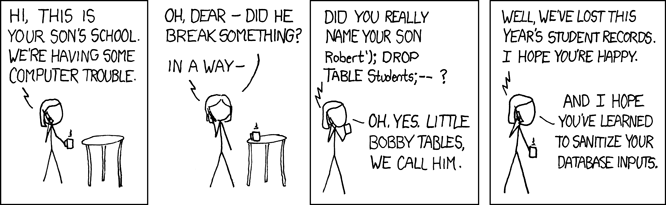
\includegraphics[width=\textwidth]{bobbytables.png}
\end{center}
\vspace{-3mm}
\caption{\url{https://xkcd.com/327/}}
\end{figure}

When done maliciously, attackers enter characters or sequences of characters which are commonly used to escape a string.
The input which follows would then be run as code on the victim's system.
The method for preventing against injection attacks is called \textsl{sanitisation},
which is simply a process of removing dangerous or unnecessary characters from a user's input.

\subsection{Firewalls}
A firewall is a piece of networking software which is designed to protect a computer system against unwanted traffic.
Firewalls scan incoming and outgoing network packets and are able to drop the packet if it is deemed unwanted.
Firewalls can be configured by a set of rules defining which traffic is unwanted.
A firewall rule could specify that a computer system drop all packets destined for port 80 or all packets not destined for port 80.
They may also be configured to support more advanced packet filtering.

From our perspective the primary advantage of a firewall is to prevent traffic which we did not intend.
If we are hosting a web server, only allowing traffic on port 80 and port 443 is desirable,
and prevents users accessing a database on the server which we forgot to password protect.
The principle for firewalls is to block by default and allow when required.

\subsection{Dependency Management}
Modern software has a lot of dependencies.
Each new dependency a software adopts is a new potential attack surface.
Relying on software which is automatically updated is dangerous,
the authors can at any point inject malicious code into your system.
There is a particularly interesting recent example of dependency injection which is worth reading about~\cite{color-js}.

One simple practice to help prevent against dependency injection is by using lock files.
Most package managers generate lock files when installing software.
Lock files keep track of the exact version of a library that is installed.
If you ask a package manager to install version >=2.4.0 of a library and it actually downloads version 2.5.6,
this will be tracked in the lock file.
Additionally, lock files track the hash of the dependency so that if someone attempts a dependency injection,
the code change will be noticed by the package manager.
Lock files should be tracked in version control and updated periodically when a safe and tested version of a dependency is released.

\section{Conclusion}
We have looked at a few guiding principles for designing and developing secure software.
This list of principles is incomplete, security requires constant consideration.
Software security is an ongoing arms race for which we are all currently unqualified to enlist.
Secure yourself as best you can and, when you are in doubt,
consult with or hire an expert.

\appendix
\section{Original Security Design Principles}\label{all-principles}

\paragraph{Saltzer and Schroeder}
\begin{enumerate}
    \item Economy of mechanism \dotfill Principle of KISS
    \item Fail-safe defaults \dotfill Principle of Least Privilege
    \item Complete mediation \dotfill Not covered
    
    \hspace{0.5em} Access to resources must \textsl{always} be authorised.

    \item Open design \dotfill Principle of Open Design
    \item Separation of privilege \dotfill Not covered
    
    \hspace{0.5em} No one user account or role should hold too much power.

    \hspace{0.5em} Consider multi-role authentication where appropriate.

    \item Least privilege \dotfill Principle of Least Privilege
    \item Least common mechanism \dotfill Not covered
    
    \hspace{0.5em} Minimise the amount of resources shared between users.

    \item Psychological acceptability \dotfill Principle of Usability
\end{enumerate}

\paragraph{Gasser}
\begin{enumerate}
    \item Consider Security from the Start \dotfill Implicit
    \item Anticipate Future Security Requirements
    \item Minimise and Isolate Security Controls
    \item Enforce Least Privilege \dotfill Principle of Least Privilege
    \item Structure the Security-Relevant Functions
    \item Make Security Friendly \dotfill Principle of Usability
    \item Do Not Depend on Secrecy for Security \dotfill Principle of Open Design
\end{enumerate}

\paragraph{Viega and McGeaw}
\begin{enumerate}
    \item Secure the Weakest Link
    \item Practice Defense in Depth
    \item Fail Securely \dotfill Principle of Failing Securely
    \item Follow the Principle of Least Privilege \dotfill Principle of Least Privilege
    \item Compartmentalise
    \item Keep It Simple \dotfill Principle of KISS
    \item Promote Privacy
    \item Remember That Hiding Secrets is Hard
    \item Be Reluctant to Trust
    \item Use Your Community Resources
\end{enumerate}
